\documentclass{report}
\usepackage{amsfonts,amsthm,amsmath,latexsym}
\usepackage[margin=1.5in]{geometry}
\usepackage{complexity}
\usepackage{graphicx}
\usepackage[titles,subfigure]{tocloft}
\usepackage{scribe-book}


\usepackage{caption}
\usepackage{subcaption}
\usepackage{float}

\newcommand{\CYCLE}{{\sf CYCLE~}}
\newcommand{\FPSPACE}{{\sf FPSPACE~}}
\newcommand{\N}{{\mathbb{N}}}
\newcommand{\Z}{{\mathbb{Z}}}
\newcommand{\F}{{\mathbb{F}}}

%% For xy matrix
\input xy
\xyoption{all}
\CompileMatrices

\usepackage{tikz}
\usetikzlibrary{arrows}

\usetikzlibrary{calc,through,backgrounds,decorations.pathmorphing}

% Shows lecture titles and sections. Set 0 to list only chapters.
\setcounter{tocdepth}{1}

\begin{document}
\newpage
\setcounter{page}{1}
\pagenumbering{roman}  % Roman numbering in intro portion.
\begin{center}
{\bf \Huge Preface}         
\end{center}

\noindent
Matter to be entered here.

\newpage
\listofscribe          % For automatic scribe list generation.

\newpage
\tableofcontents

\setcounter{page}{1}
\pagenumbering{arabic}  % Arabic page numbering for lectures.

% Autogenerated using Makefile. DO NOT EDIT
\newpage \Lecture{Dinesh K.}{Jan 10, 2012}{4}{Quest for Structure in Counting Problems}
%\theme{Between $\P$ and $\PSPACE$.}
%\lectureplan{Counting problems and their structural complexity. Various attempts to develop the theory and the class $\#\P$. Basic containments.}

%We have seen several decision problems where we are interested in knowing the
%existence or non-existence of objects satisfying a certain property. An
%equally interesting question would be to ask the count of such objects. Such
%problems are called as counting problem.

In the previous lecture, we saw that the counting problem can be as hard as (or 
harder than) the decision problem as given an algorithm for counting problem
the decision problem reduces to just checking the count to be zero or not. We
also saw an easy decision problem \CYCLE whose counting version \#\CYCLE is
\NP-hard (by reduction from {\sf HAMCYCLE}) implying that easy decision
problems can also have corresponding counting problems hard. We also argued
that talking about counting problems still makes sense as the count value,
though exponential, can still be represented in polynomial number of
bits.

In this lecture, we will study counting problems and understand their
structural complexity. We shall also make attempts to develop the theory of
complexity classes capturing the counting problems (especially \#\P). We shall
also discuss their basic containments.

\section{Preliminaries}
Firstly, we fix our computation model where we have a Turing machine with an
input tape, work tape and an output tape. We are interested in the resources
used by the Turing machine - space (considering only the work tape) and time.

We want to capture the notion of counting formally. One such way is to see it
as computing a function $f : \Sigma^* \to \N$ where $\Sigma=\{0,1\}$ which
gives an integer value. So, how can we capture the notion of computing a
function? There are two possible ways of capturing function computation.
\begin{description}
\item[Variant 1] We say that a function $f$ is computable if each bit of the
output can be computed in some decision complexity class $\calC$.
\item[Variant 2] $f$ is computable if the value of the function computation
can be written down within the resource bounds.
\end{description}

Analogous to the decision problems, we define complexity classes for function
computation problems. A natural extension of \P~is \FP~ which is defined as
\begin{center}
\FP = $\{f \left | \right . f:\Sigma^* \to \N, f(x) \text{ for any } x \in
\Sigma^* \text{ can be written down in } poly(|x|) \text{ time}\}$
\end{center}

Now, we shall plugging in the two variants of function computation and see
which of them is more appropriate.

\section{Comparing the variants}
We quickly observe that the first and the second variant really coincides when we are talking
about deterministic computations. Let us do this analysis by attempting the definition of $\FP$.
Following the first variant $f \in \FP$ iff there exists an algorithm that can
compute each bit of $f$ in class \P. But since the algorithm is deterministic, this is  
equivalent to saying that $\forall~i$, the language defined by the $i^{th}$ bit 
$$L_{f_i} = \{ x : (f(x))_i = 1 \} \in \P$$
On the other hand, if each bit can be computed in polynomial time 
and since the count value can be represented in polynomial number of bits, for
evaluation, we just run a polynomial time algorithm polynomial times
which is still a polynomial. Hence we have an algorithm that satisfies the 
second variant.

Hence for deterministic polynomial time computation both variants are equivalent.
We can define other classes for deterministic computation 
like {\sf FL}(log space bounded function computation), \FPSPACE(polynomial
space bounded function computation). Containments of these classes are
analogous to their decision versions. We leave the proof as an exercise.

\begin{lemma}
${\sf FL} \subseteq \FP \subseteq \FPSPACE$
\end{lemma}

Now we turn into the non-deterministic world. 
Following variant 1 of definition of function computation, we must have each
bit computable in class \NP. But variant 2 is not useful because an non-deterministic 
poly time Turing machine by our model is not set to output a value. How can we
capture the function computation for a non-deterministic machine for decision
problems which works by guess-verify mechanism?

Now, consider the non-deterministic algorithm
we had for \SAT, which does guessing of an assignment and verifying it. 
We can observe the following additional property.
\begin{observation}
Number of satisfying assignments is exactly equal to the number of accepting
paths.
\end{observation}
This leads to the question as to whether this is accidental or is there some
hidden structure? It also assigns a function value to the non-deterministic Turing machine.
This motivates us to give a new model, for us to call $f$ is computable by a non-deterministic polynomial time Turing machine.

\begin{definition}
$f$ is $\#\P$ if there exists a non-deterministic Turing machine $M$ running in time $p(n)$ such that 
$\forall x \in \Sigma^*$, $f(x) = \left| \{ y \in \{0,1\}^{p(n)}  : M \textrm{ accepts on path $y$ } \} \right|$.
\end{definition}

\begin{remark}
The RHS is also the number of accepting paths of $M$ on $x$ if the lengths of all paths are equal to $p(n)$.
We remark that this can be achieved without loss of generality. That is, from an arbitrary TM $M$, we can get to a new TM $M'$ which has the same number of accepting paths, such that the number of accepting paths on any input $x$ remains the same. We recall our observation that for length of all non-deterministic paths of an \NP~machine on any input can be made equal without changing the accepted language\footnote{In particular, we showed that a language $A \in \NP$ if and only if there is a language $B \in \P$ and a polynomial $p(n)$ such that $x \in A \iff \exists y \in \{0,1\}^{p(n)} : (x,y) \in B$} . But this construction makes the language accepted the same, and need not keep the number of accepting paths the same. We modify it slightly to achieve our goal.  Indeed, if a path is shorter than $p(n)$ bits and decided A/R, we extend it to the required length using a binary tree of paths rooted at that node and make the left most path (in this binary tree) report A/R respectively and make all other paths reject. The number of accepting paths does not change due to this construction.
\end{remark}

\begin{remark}
Try this as an exercise. Initiate the thought process on : how does this definition compare with variant 1? What does computing/testing each bit to be 0/1 mean?
\end{remark}

%\begin{proof}
%Recall that, 
%\begin{center}
%$ \calL \in \NP \iff \exists \calB \in \P \text{ and a polynomial } p(n)
%\text{ such that} $ 
%$(x \in \calL \iff \exists y \in \{0,1\}^{p(n)}, (x, y) \in \calB )$
%\end{center}
%Hence  a non-deterministic machine $N$ for $\calL$ just need to guess $p(n)$
%bits and run the verifier to validate the guess. Hence every non-deterministic
%path will be of length $p(n)$.
%\end{proof}
%Hence our observation actually follows from the definition. This gives us a
%better characterisation.

%\begin{definition}
%$f$ is computable by a non-deterministic Turing machine $M$ running in 
%ime $p(n)$ if $ \forall x \in \Sigma^*, f(x) = |\{ y \in \{0,1\}^{p(n)} | 
% \text{ accepts on path } y \}|$. The class of functions for which such 
%non-deterministic Turing machines exists is called \#\P (``sharp P")
%\end{definition}

Counting version of \SAT~denoted as \#\SAT~can be defined as 
\[ \#\SAT(\phi) = |\{ \sigma | \phi(\sigma) = 1, \sigma \text{ is a boolean
assignment to variables in } \phi \}| \]
It follows from our observation that $\#\SAT \in \#\P$, since we can give a
non-deterministic machine (i,e. a machine for \SAT) where number of accepting
paths equals to the number of satisfying truth assignments. It can also be
shown that $\#\CYCLE \in \#\P$.

\begin{claim}
$\#\CYCLE \in \#\P$
\end{claim}
\begin{proof}
Following is a non-deterministic Turing machine $N$, such that number of
cycles equals number of accepting paths.

$N$ = `` On input $G$,
\begin{enumerate}
\item Guess subsets $V' \subseteq V(G)$ and $E' \subseteq E(G)$ 
non-deterministically.
\item Accept iff $V', E'$ form a simple cycle. "
\end{enumerate}

Now it follows that $\#\CYCLE(G) = |\{ \# \text{ of accepting paths of } N
\text{ on } G \}|$ since any cycle can uniquely be characterised by an edge set
and a vertex set.
\end{proof}

\section{Basic Containments}
In the functional world, we have the following scenario.
\begin{center}
\FPSPACE \\
$\vert$ \\
\FP \\
$\vert$ \\
{\sf FL }
\end{center}

So where does set of functions, $\#\P$ lie? We will argue that $\#\P$ lies between 
\FP and \FPSPACE thus replicating the picture in the decision world.
\begin{lemma}
$\#\P \subseteq \FPSPACE$
\end{lemma}
\begin{proof}
Given a non-deterministic poly time Turing machine $M$ computing function $f$,
we just need to do a simulation in deterministic poly space. This can be done by
simulating $M$ over all non deterministic paths while reusing space across the
paths. Since length of any path is polynomially bounded, space used will also
be polynomial. In the process we need to keep the count of accepting paths
which can be $\le 2^{p(n)}$ but still representable with $p(n)$ bits in
binary. Hence space requirement is only polynomial in input length.
\end{proof}

\begin{lemma}
$\FP \subseteq \#\P$
\end{lemma}
\begin{proof}
Given an $\calL \in \FP$, there exists a deterministic Turing machine $M$ which
$\forall x \in \calL$ writes $f(x)$ in $p(n)$ time where $p$ is a polynomial
and $n = |x|$. To show that $\calL \in \#\P$, we need to construct a
non-deterministic  such that
\begin{center}
No of accepting paths = $f(x)$.
\end{center}
$N$ can compute $f(x)$ by simulating $M$. Let the value obtained be $k$. Now,
$N$ must have exactly $k$ accepting paths. This can be ensured by guessing
$\lceil \log k \rceil$ bits and accepting all the paths whose address have
binary representations  $\le k$ and rejecting the remaining paths.

$N$ runs in poly time since $f(x)$ computation (simulation of $M$) takes only
polynomial time. Even though $f(x)$ is exponential, number of bits guessed is
$\lceil \log f(x) \rceil$ which will be polynomial in $n$. Hence depth is
polynomially bounded. Also number of accepting paths equals $f(x)$ by
construction. Thus $N'$ is a \#\P machine accepting $\calL$. Hence $\calL =
L(N') \in \#\P$.
\end{proof}

\begin{figure}[htp!]
\centering
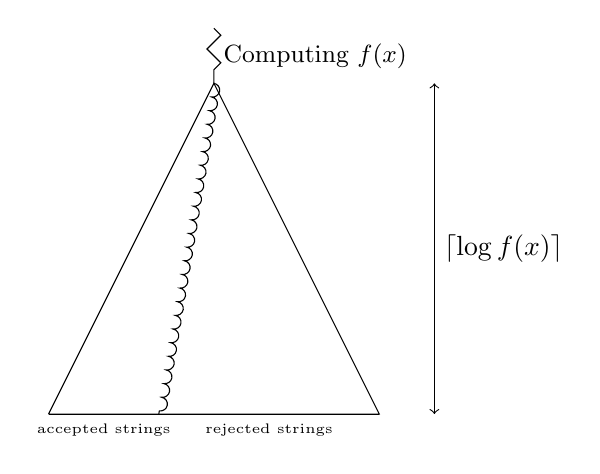
\begin{tikzpicture}[scale=0.7]
\coordinate (T) at (3,7);
\coordinate (A) at (0,0);
\coordinate (B) at (6,0);
\coordinate (C) at (3,6);
\coordinate (M) at (2,0);
\draw [decorate,decoration=zigzag] (T) -> (C) node[midway,right]
{ {\small Computing $f(x)$ }};
\draw (A) -- (M) node[midway,below] { {\tiny accepted strings}} ;
\draw (M) -- (B) node[midway,below] { {\tiny rejected strings}} ;
\draw (A) -- (B) -- (C) -- (A);
\draw [decorate,decoration=bumps] (C) -> (M);
\draw [<->] (7,0) -- (7,6) node[midway,right] {$\lceil \log f(x) \rceil$};
\end{tikzpicture}
\end{figure}

It can be observed that if function computation can be done in polynomial time
then $\P = \NP$. This is because solving decision problem amounts to checking
if the corresponding counting function gives a non zero value or not hence
making decision problem easy if function computation is in \P. 
\begin{lemma}
$\#\P = \FP \implies \P = \NP$
\end{lemma}

An interesting question would be to ask if the converse it true? That is 
\begin{center}
Does $\P = \NP \text{ imply }  \#\P = \FP ?$
\end{center}
We will address this and show a weaker implication (that is, based on slightly stronger LHS) in the next lecture.


\newpage \Lecture{Prasun Kumar}{Jan 12, 2012}{5}{$\FP$ vs $\#\P$ question}
%\theme{ Between $\P$ and $\PSPACE$.}
%\lectureplan{ $\FP$ vs $\#\P$ question, a counter part in the decision world. The class PP. PP vs P is equivalent to FP vs $\#\P$.}

We know $(\#\P = \FP) \implies (\P = \NP)$. In the last lecture we left the question about the converse.
i.e., is it true that, $(\P = \NP) \implies (\#\P = \FP)$?

In this lecture, we will show a weaker version of the above containment.
We will define a new class of languages $\PP$ (probabilistic polynomial time)
in decision world, that contains $\NP$, and will show that if we make a stronger assumption $\PP = \P$ (seemingly stronger than $\NP = \P$) we get the required implication.  We will show in particular that $\PP = \P \iff \#\P = \FP$.

\section{Complexity Class \PP}
For exploring the complexity class, we revisit the definition of $\NP$.
With respect to a "branching" Turing machine(NTM) (which can branch at each computation by using a guess bit), we have two different classes of languages as follows, which differs in their acceptance conditions. We denote for a machine $M$, by $\#acc_M(x)$ as the number of accepting paths. Let the machine run for $p(n)$ time on each path.
\begin{itemize}
\item $\NP$ = $\{$L : $\exists$ branching TM $M_1$, x $\in$ L $\iff \#acc_{M_1}(x) \ge 1 \}$.
\item $\coNP$ = $\{$L : $\exists$ branching TM $M_2$, x $\in$ L $\iff \#acc_{M_2}(x) \ge 2^{p(n)} \}$.
\end{itemize}

In terms of number of accepting paths on input $x$, the above classes
represent the extremes.  On one side, in $\NP$ we talk of atleast one
accepting path, and on the other side, in $\coNP$ we talk of all
accepting paths. To understand the structure of these classes we can
ask the variant of this as : what different class of languages do we
get if we set the accepting condition as the number of accepting paths
being more than a fraction of the total number of paths on input {\em
  x}. A simpler situation is to consider the fraction to be half and the
corresponding class of languages is called \PP (probabilistic
polynomial) which is defined as follows. We will come across other variants in
the later lectures.

\begin{definition}
$\PP$ =$\{$L : $\exists$ NTM $M$, x $\in$ L $\iff \#acc_{M_1}(x) > 2^{p(n)-1} \}$
\end{definition}

We first understand this complexity class with respect to the other ones we have already seen. We start with the following proposition.

\begin{proposition}
\label{prop}
$\NP \subseteq \PP$.
\end{proposition}
\begin{proof}
Let $L \in \NP$  via a nondeterministic turing machine $M$,  $ x \in L \iff M$ has atleast one accepting path on $x$. 
Our aim is to give another turing machine $M'$ for the same language $L$ such that
$x \in L \iff M'$ has more than half of the total number of paths as accepting paths on $x$.\\
Description of $M'$ (on input $x$):
\begin{enumerate}
\item Simulate $M$ on $x$.
\item If $M$ accepts then choose one bit nondeterministically and accept in both branches.
\item If $M$ rejects then choose one bit nondeterministically,accept in one branch and reject in other.
\end{enumerate}

As we remarked in the last lecture, we can assume without loss of generality that the height of computation tree of $M$ on $x$ is exactly $p(n)$ for some polynomial $p$. Since the total number of paths for $M'$ on input $x$ is $2^{p(n)+1}$, it suffices to prove that $x \in L \iff \#acc_M(x) > 2^{p(n)}$.
Let $x \in L$. Since $M$ has at least one accepting path on $x$. Since $M'$, by construction, creates an imbalance (in count) between the number of accepting and rejecting paths precisely when $M$ accepts,  the number of accepting paths in $M'$ will be more than the number of rejecting paths. Thus $\#acc_M(x) > 2^{p(n)}$. \\
If  $x \not\in L$, all paths reject in $M$ on input $x$, and thus  number of accepting and rejecting
paths in $M'$ on input $x$ are exactly equal and each of themsame is equal to $2^{p(n)}$.
\end{proof}

A similar proof will also show that $\coNP$ is contained in
$\PP$. Thus we have the following containment relationship among
different classes of languages
 
\begin{center}
\PSPACE \\ 
$\vert$ \\
\PP \\
$\vert$ \\
\NP \\
$\vert$ \\
\P
\end{center}

Now we will prove the main theorem of the lecture which characterizes the $\FP$ vs $\#\P$ question in the decision world.

\begin{theorem}
 $(\#\P = \FP) \iff (\PP = \P)$
\end{theorem}
\begin{proof}
($\Rightarrow$) Assume $\#\P = \FP$, our aim is to prove $\PP = \P$. The reverse containment follows since we know $\NP \subseteq \PP$ by proposition\ref{prop}. Now we show that $\PP \subseteq \P$ . Let $L \in \PP$
via a machine $M$ running in time $p(n)$ for some polynomial $p$, such that $x \in L \iff \#acc_M(x) > 2^{p(n)-1}$.
Define the function, $f(x) = \#acc_M(x)$. By definition $f \in \#\P$ and hence $f \in \FP$. There is a deterministic polynomial time Turing machine $N$ which on input $x$ outputs the value of $f(x)$. Given an $x$, to test whether it is in $L$ or not, it suffices to test whether whether the MSB of the binary representation of $f(x)$ is 1 or not. This can be done by simply running the machine $N$ on $x$ and testing the MSB of the output. Hence $L \in P$.

($\Leftarrow$) Assume $\PP = \P$, our aim is to prove $\#\P = \FP$. The reverse direction is easy. $\FP \subseteq \#\P$ as we argued in the last lecture. To show the forward direction, let $f\in \#\P$ via $M$ such that $\forall x \in \Sigma^*$, $f(x)=\# accept_M(x)$. Note that the naive approach to compute $f(x)$ is to compute the number of accepting paths in computation tree of height $p(n)$ will take exponential time. But it suffices to find the minimum $0 \le k \le 2^{p(n)}$ such that :
\begin{equation}
\label{eqn}
k+\#acc_M(x) > 2^{p(n)}
\end{equation}
Indeed, the minimum is achieved when $k = k_{min} = 2^{p(n)} - \#acc_M(x) + 1$. Thus $\#acc_M(x) = 2^{p(n)} - k_{min} +1$. This is an indirect way of finding out $\#acc_M(x)$ and we are moving towards using our assumption that $\PP = \P$.

We have  search problem in hand; to search for the minimum $k$($k_{min}$) satisfying equation (\ref{eqn}). We do this by binary search over the range $0 \le k \le 2^{p(n)}$. We solve the decision problem first. {\sf Given $x$ and $k$, check if $k+\#acc_M(x) > 2^{p(n)}$}.

For this, we construct an another Turing machine $N$ such that the number of accepting paths is exactly $k+\#acc_M(x)$ and the total number of paths is $2^{p(n)+1}$. Assume such a construction exists. Define a language $A \subset \Sigma^*$ such that $x \in A \iff k+\#acc_M(x) > 2^{p(n)}$. Thus $x \in A \iff \#acc_N(x) > 2^{p(n)}$. This implies that $A \in PP$ (via the machine $N$ !) and hence $A \in P$ by assumption. Given $x \in \Sigma^*$ we can test if $k+\#acc_M(x) > 2^{p(n)}$ by testing if $x \in A$ or not, which can be done in polynomial time. Now we can do this construction and simulation through a binary search in order to find the minimum value of $k$ that satisfies our inequality.

To complete the proof, we give the construction of $N$ (for a given $k$). 
We first construct a machine $M_k$ that runs in time $p(n)$ and has exactly $k$ accepting paths. 
We slightly modify the idea in the previous lecture to do this. Let $\ell = \lceil \log k \rceil$.
The machine $M_k$ guesses a $y \in \{0,1\}^{p(n)}$ and {\em accepts} if the first $\ell$ bits of $y$ in binary represents a number less than $k$ and the last $p(n)-\ell$  bits is all-zero (lexicographically first path) and {\em reject} otherwise.

We combine $M_k$ and $N$ (both using exactly $p(n)$ non-deterministic bits), to get the machine $N$. The machine $N$ on input $x$ guesses $1$ bit and on the $0$-branch it simulates $M_k$ on $x$ and on the $1$-branch it simulates $M$ on $x$. Clearly $\#acc_N(x) = \#acc_{M_k}(x) + \#acc_{M}(x) = k+\#acc_{M}(x)$. The length of each path is exactly $p(n)+1$ and hence total number of paths is $2^{p(n)+1}$.
\end{proof}






\bibliographystyle{abbrv}
\bibliography{references}

\end{document}
